


\begin{table}[]
    \centering
    \begin{tabular}{lll}
    \hline
    Parameter                    &  & Value \\ \hline
    Episode Lenght               & \( H \) & 1000  \\
    World height                 &  & 25    \\
    World width                  &  & 25    \\
    Resources respawn prob.      &  & 0.01  \\
    Inital Coin endowment        &  & 0     \\
    Iso-elastic utility exponent &  \(\eta\)& 0.23  \\
    Move labor                   &  & 0.21  \\
    Gather labor                 &  & 0.21  \\
    Trade labor                  &  & 0.05  \\
    Build labor                  &  & 2.1   \\
    Base build payout            &  & 10    \\
    Max skill multiplier         &  & 3     \\
    Max bid/ask price            &  & 10    \\
    Max bid/ask order duration   &  & 50    \\
    Max simultaneous open orders &  & 5     \\
    Tax period duration          & M & 100   \\
    Min bracket rate             &  & 0\%   \\
    Max bracket rate             &  & 100\% \\ \hline
    \end{tabular}
    \caption{\label{tab:hyperparameter_env}Hyperparameters for the environment.}
\end{table}

\begin{table}[]
    \centering
    \begin{tabular}{lll}
    \hline
    Parameter                    &  & Value \\ \hline
    Training Algorithm               &  & ppo \\
    Number of Agents & N & 4\\
    Number of parallel environment replicas                &  & 60    \\
    Sampling horizon (steps per replica)               & h & 200   \\
    Train batch size && 3000\\
    SGD minibatch size     &  & 500 \\
    Number SGD iter      &  & 10    \\
    CPUs                   &  & 2  \\ \hline
    Learning rate                & Lr & 3e-4   \\
            Learning rate schedule (phase 1)      &  & [[0, Lr], [10M, Lr], [30M, 0]] \\
        Learning rate schedule (phase 2)      &  &[[35M, Lr], [50M, 1e-6]]\\
    Entropy regularization coefficient                  &  & 1e-4 \\
    Gamma                 & $\gamma$ & 0.99  \\
    GAE lambda           &  & 0.9    \\
   Gradient clipping parameter         &  & 0.25    \\
    Value function loss coefficient             &  & 0.05   \\ \hline
    Number of fully-connected layers  &  & 2   \\
    Agents get full spatial observation &  & False     \\
    Agent spatial observation box half-width          &  & 5   \\ \hline
    Phase one training duration &  & 35M  \\
    Phase one energy warm-up constant & $\vartheta$ & 10000  \\
    Phase two training duration  &  &  150M \\ \hline
    \end{tabular}
    \caption{\label{tab:hyperparameter_train}Hyperparameters for the Training.}
\end{table}

\begin{table}[]
    \centering
    \begin{tabular}{ll}
    \hline
    Variable Name                                 & Dimension                   \\ \hline
    world Map                                     & (7, 11, 11)                    \\ 
    world-idx\_map                                & (2, 11, 11)               \\ 
    world-loc-row                                 & (1,)                         \\ 
    world-loc-col                                 & (1,)                         \\ 
    world-inventory-Coin                          & (1,)                         \\ 
    world-inventory-Stone                         & (1,)                                    \\ 
    world-inventory-Wood                          & (1,)                                    \\ 
    time                                          & (1, 1)                                   \\ 
    Build-build\_payment                          & (1,)                                     \\ 
    Build-build\_skill                            & (1,)                                     \\ 
    ContinuousDoubleAuction-market\_rate-Stone    & (1,)                                     \\ 
    ContinuousDoubleAuction-price\_history-Stone  & (11,)                                    \\ 
    ContinuousDoubleAuction-available\_asks-Stone & (11,)                                    \\ 
    ContinuousDoubleAuction-available\_bids-Stone & (11,)                                    \\ 
    ContinuousDoubleAuction-my\_asks-Stone        & (11,)                                    \\ 
    ContinuousDoubleAuction-my\_bids-Stone        & (11,)                                    \\ 
    ContinuousDoubleAuction-market\_rate-Wood     & (1,)                                     \\ 
    ContinuousDoubleAuction-price\_history-Wood   & (11,)                                    \\ 
    ContinuousDoubleAuction-available\_asks-Wood  & (11,)                                    \\ 
    ContinuousDoubleAuction-available\_bids-Wood  & (11,)                                    \\ 
    ContinuousDoubleAuction-my\_asks-Wood         & (11,)                                \\ 
    ContinuousDoubleAuction-my\_bids-Wood         & (11,)                                    \\ 
    Gather-bonus\_gather\_prob                    & (1,)                                     \\ 
    action\_mask                                  & (50,)                                    \\ \hline
    \end{tabular}
    \caption{\label{tab:full_obs} Full observation space.}
\end{table}




\begin{algorithm}
  \caption{Agents Learning Loop.}\label{alg:training}
  \begin{algorithmic}
    \Require Sampling horizon $h$ and tax period $M$
    \Require On-policy learning algorithm $\mathcal{A}$ \Comment{PPO}
    \Require Stopping criterion \Comment{i.e. utility convergence}
    \Ensure Trained agent policy weights $\theta$
    
        \State $s, \mathbf{o} \, \gets \, s_0, \mathbf{o_0}$ \Comment{reset episode}
        \State $\theta \, \gets \, \theta_0$
        \State $D \gets \{\}$ \Comment{reset transition buffer}
        
        \While{training}
            \For{ $ t = 0,1,...,h$}
                \State $\mathbf{a} \gets \mathbf{\pi}(\cdot|\mathbf{o}, \theta)$
                \State $s', \mathbf{o}', \mathbf{r} \gets$ Env.step($s, \mathbf{a}, \tau$)
                \If{t mod $M$ = $M -1$}
                    \State $s', \mathbf{o}', \mathbf{r} \gets$ Env.tax($s'$)
                \EndIf
                \State $D\, \gets \, D \, \cup\, \{ (\mathbf{o},\mathbf{a},\mathbf{r},\mathbf{o}')\}$
                \State $s, \mathbf{o} \, \gets \, s', \mathbf{o}'$
            \EndFor
            \State Update $\theta$ using data in $D$ and $\mathcal{A}$
            \State $D \gets \{\}$
            \If{episode is completed}
                $s, \mathbf{o} \, \gets \, s_0, \mathbf{o_0}$ \Comment{reset episode}
            \EndIf
            \If{the stopping criterion has been met}
                \Return $\theta$
            \EndIf
        \EndWhile
  \end{algorithmic}
\end{algorithm}




\begin{figure}[h!]
    \centering
    \linespread{.9}
    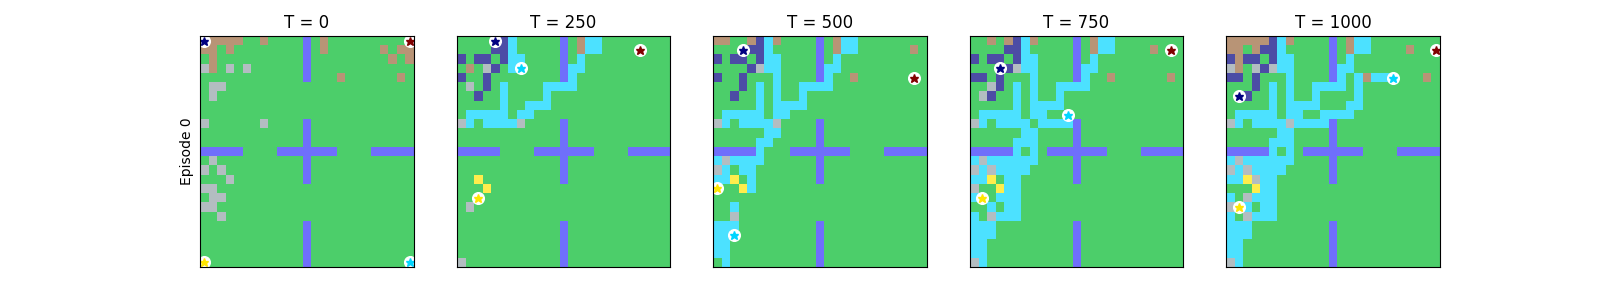
\includegraphics[width=0.95\textwidth]{Resources/imgs/Figure_1_Free.png}
    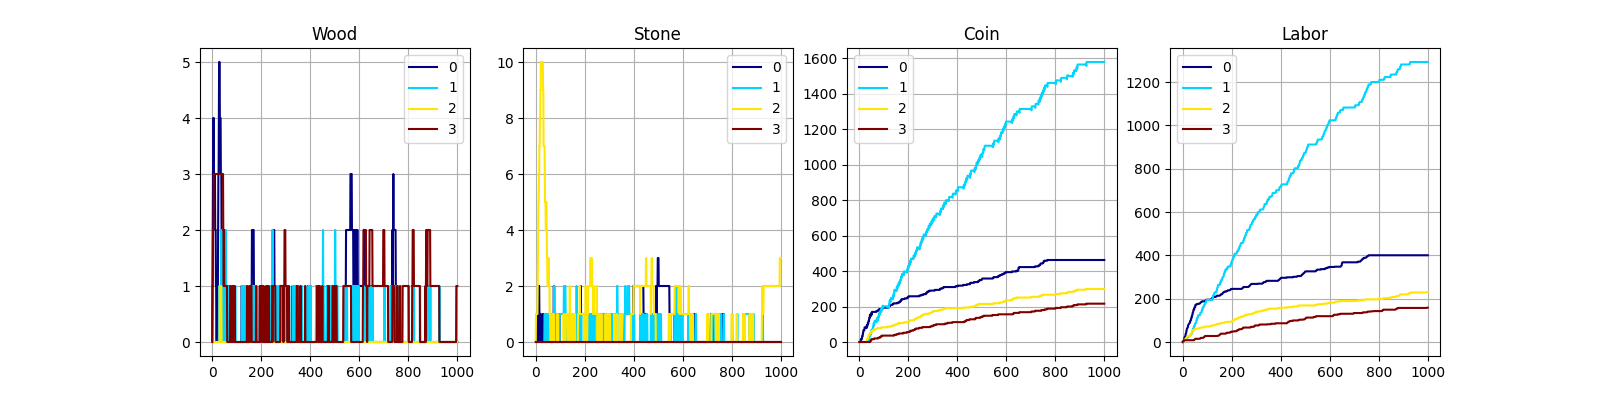
\includegraphics[width=0.80\textwidth]{Resources/imgs/Figure_2_Free.png}
    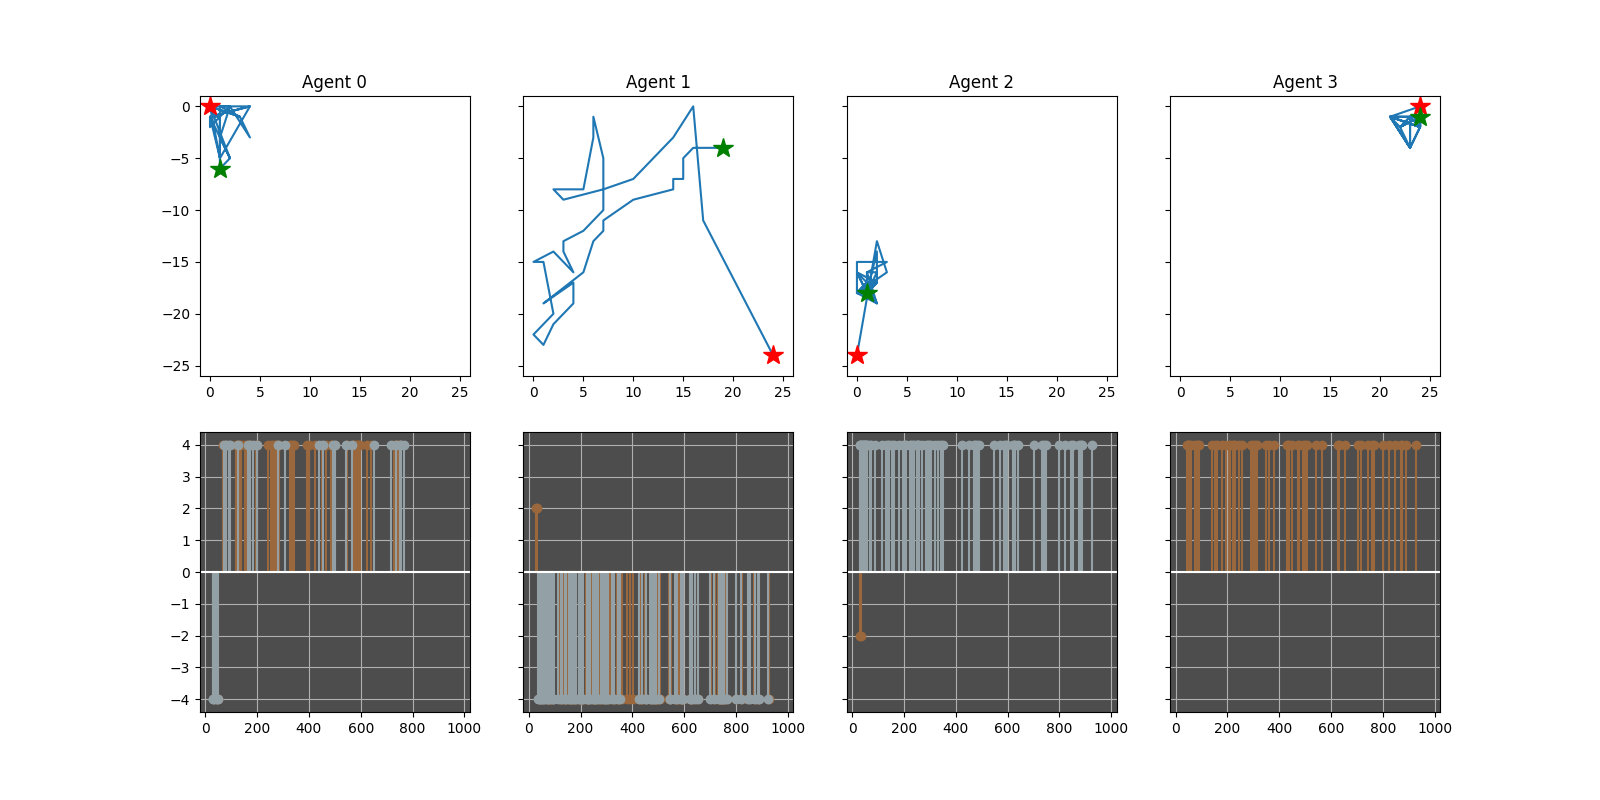
\includegraphics[width=0.80\textwidth]{Resources/imgs/Figure_3_Free.png}
    \caption[Free market full brake down: ]%
    {\label{img:Free_brakedown}Free market full brake down: \small \textit{this is a more complete overview of one random simulation crated using the weights at the end of phase 2 training for the Free market.}}
\end{figure}

\begin{figure}[h!]
    \centering
    \linespread{.9}
    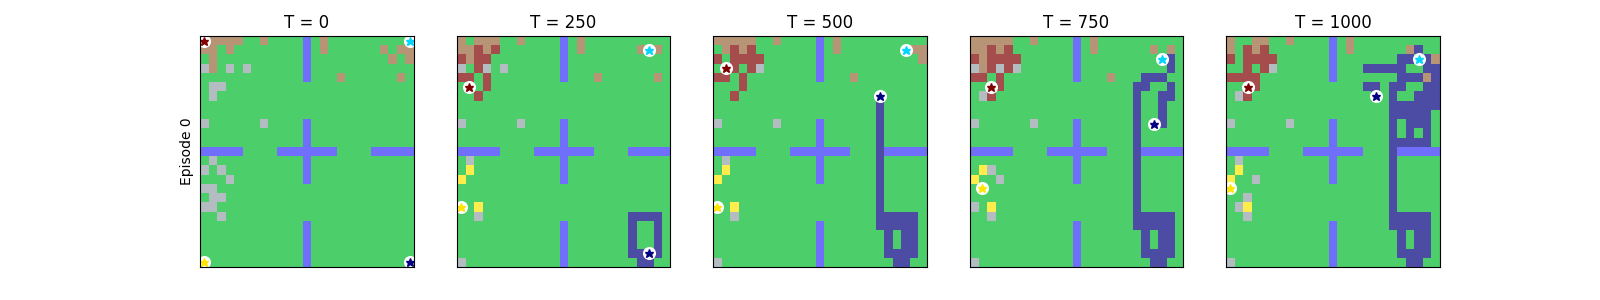
\includegraphics[width=0.95\textwidth]{Resources/imgs/Figure_1_Us.png}
    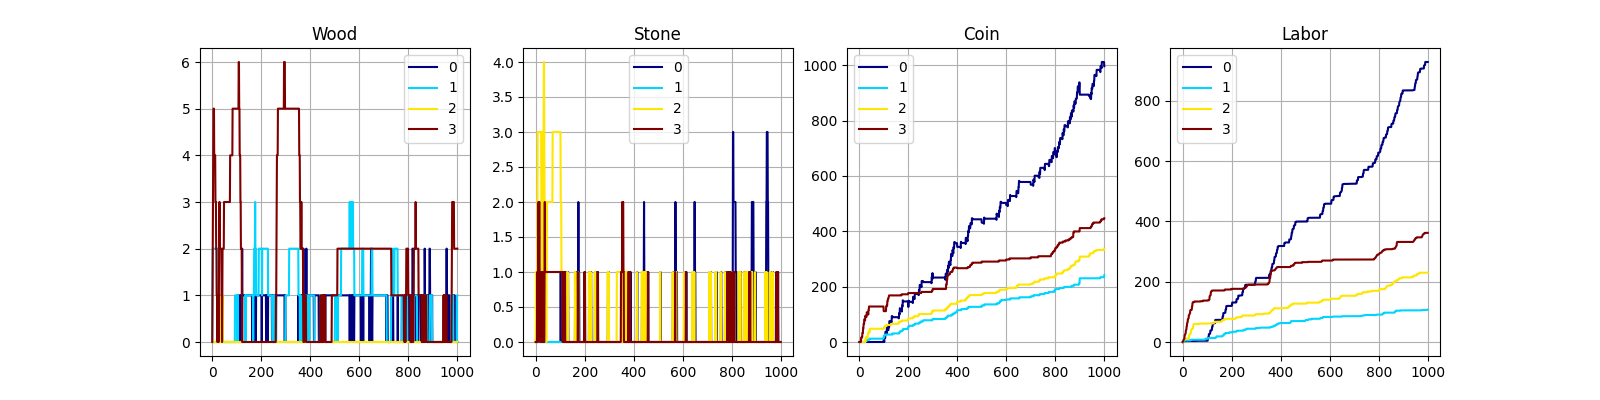
\includegraphics[width=0.80\textwidth]{Resources/imgs/Figure_2_Us.png}
    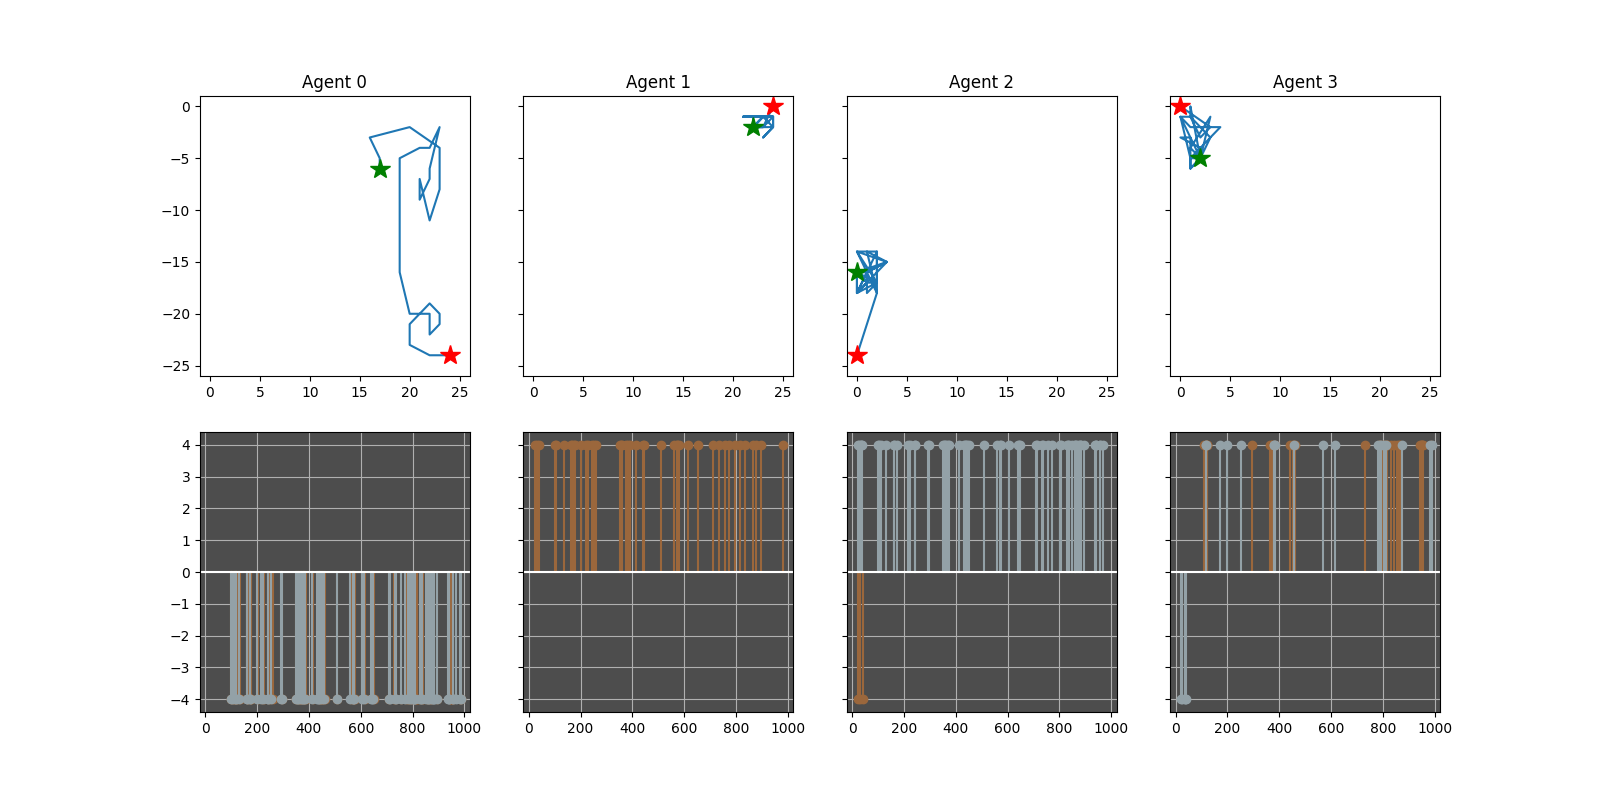
\includegraphics[width=0.80\textwidth]{Resources/imgs/Figure_3_Us.png}
    \caption[US full brake down: ]%
    {\label{img:p0_brakedown}US full brake down: \small \textit{this is a more complete overview of one random simulation crated using the weights at the end of phase 2 training for US taxation.}}
\end{figure}

\begin{figure}[h!]
    \centering
    \linespread{.9}
    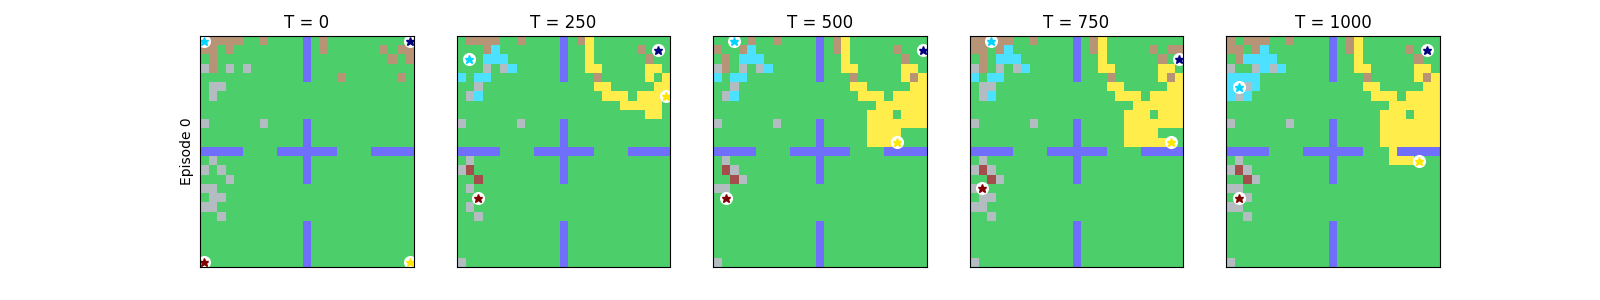
\includegraphics[width=0.95\textwidth]{Resources/imgs/Figure_1_Ita.png}
    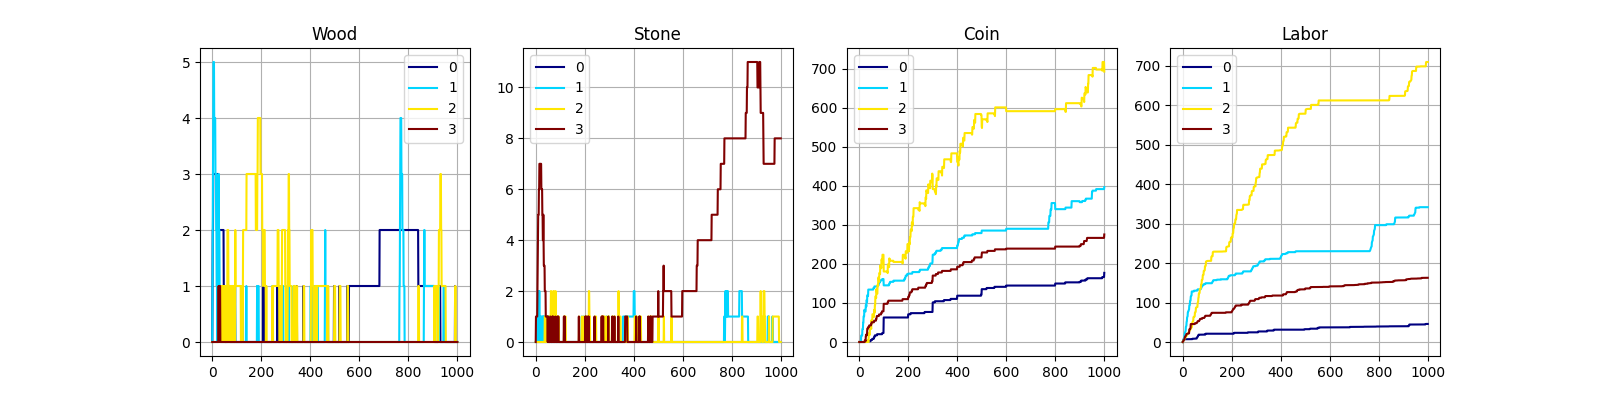
\includegraphics[width=0.80\textwidth]{Resources/imgs/Figure_2_Ita.png}
    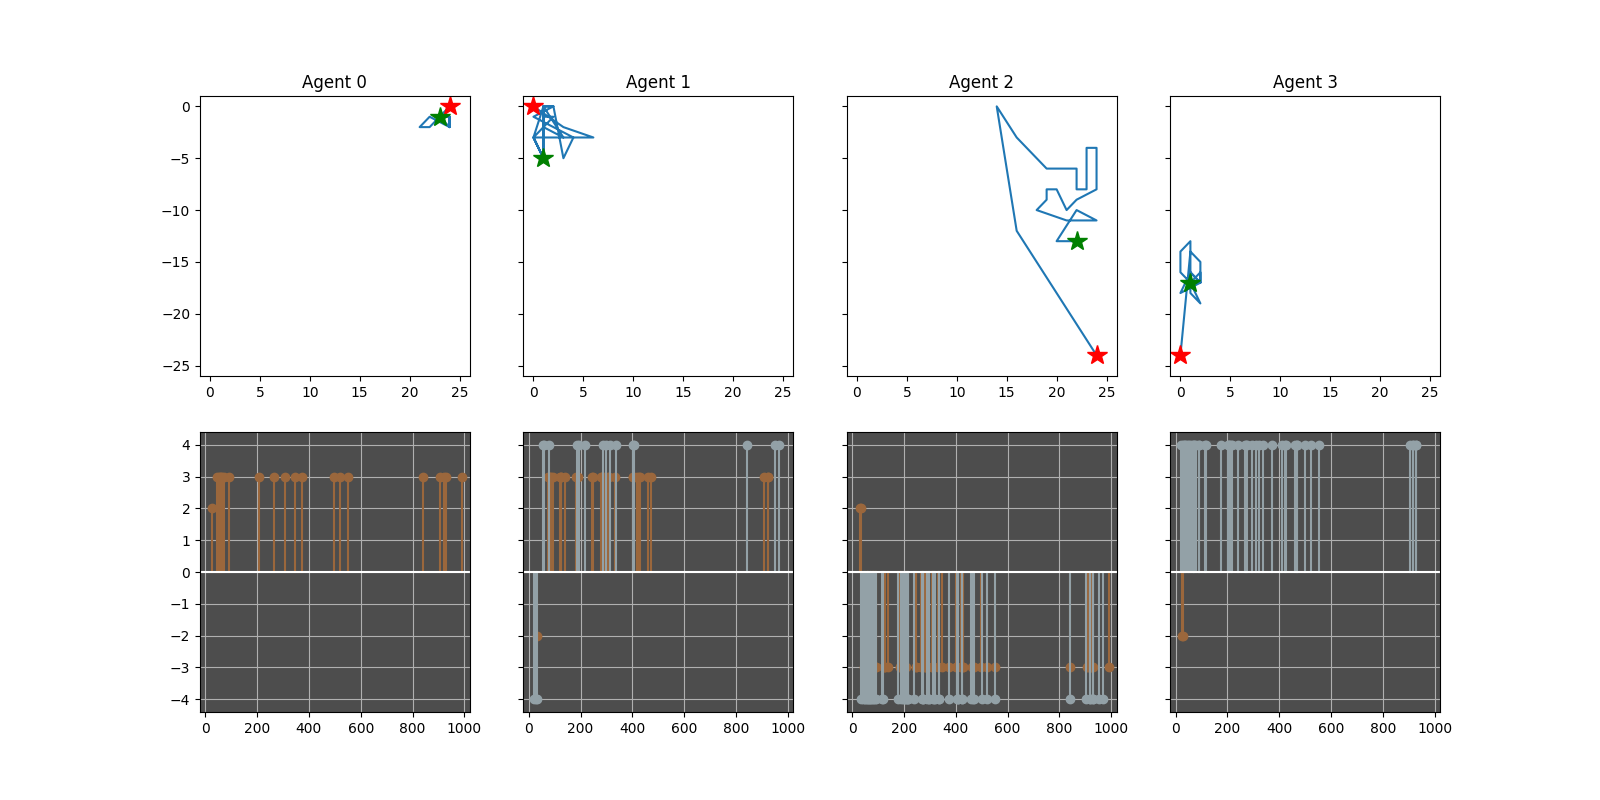
\includegraphics[width=0.80\textwidth]{Resources/imgs/Figure_3_Ita.png}
    \caption[Italy full brake down: ]%
    {\label{img:p0_brakedown}Italy full brake down: \small \textit{this is a more complete overview of one random simulation crated using the weights at the end of phase 2 training for Italian taxation.}}
\end{figure}

\begin{figure}[h!]
    \centering
    \linespread{.9}
    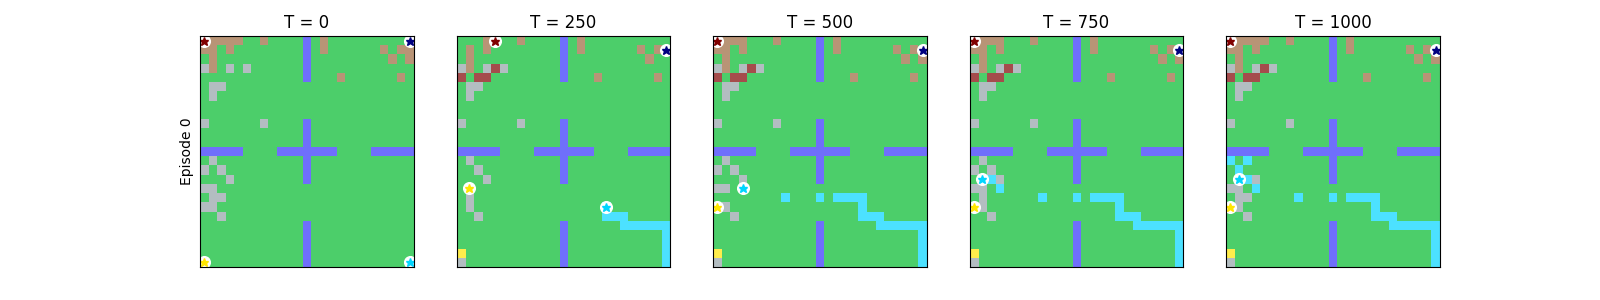
\includegraphics[width=0.95\textwidth]{Resources/imgs/Figure_1_Comm.png}
    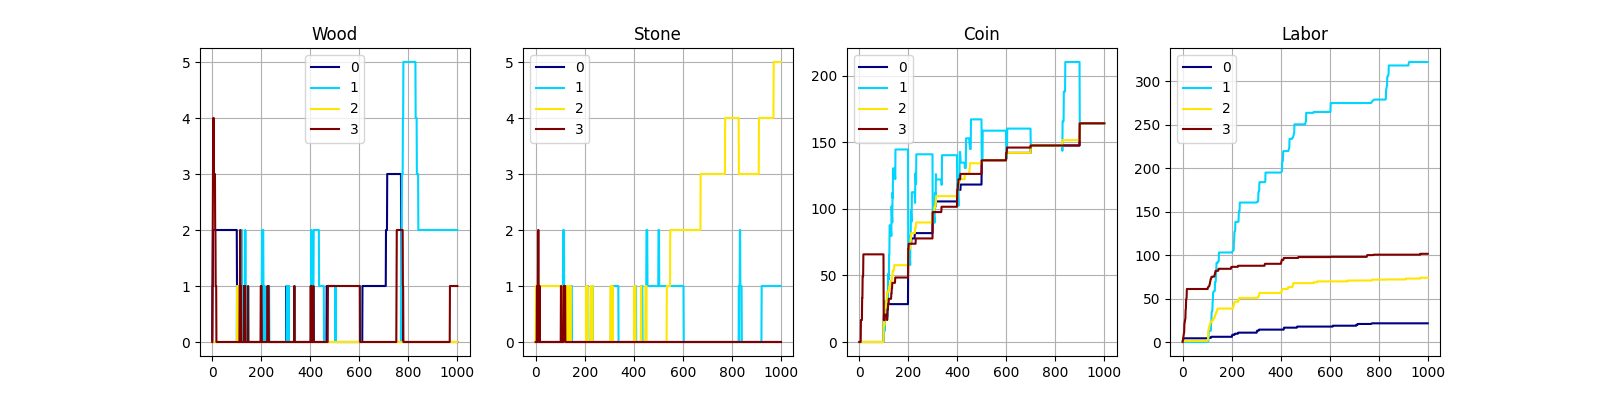
\includegraphics[width=0.80\textwidth]{Resources/imgs/Figure_2_Comm.png}
    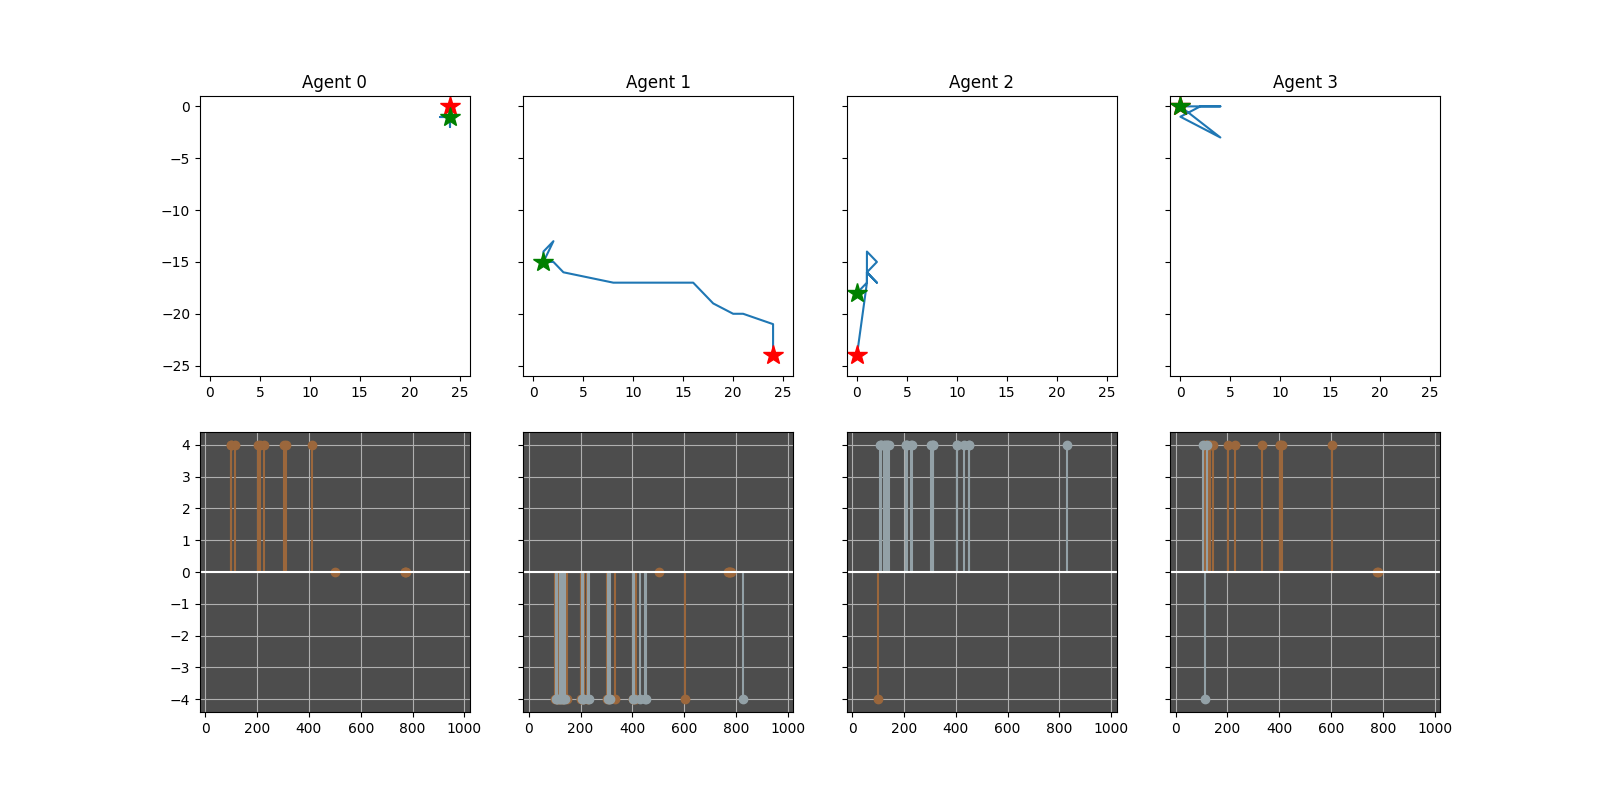
\includegraphics[width=0.80\textwidth]{Resources/imgs/Figure_3_Comm.png}
    \caption[Communism full brake down: ]%
    {\label{img:p0_brakedown}Communism full brake down: \small \textit{this is a more complete overview of one random simulation crated using the weights at the end of phase 2 training for communism.}}
\end{figure}

